\section{Analysis}
In this section we discuss the results of our analysis. We implemented a basic seq2seq model, and extended that using the approaches~\ref{mod:bos}~and~\ref{mod:onehot}. Section~\ref{sec:ref} presents a list of sources that were used to implement the models.

During the training we collected the average sentence perplexitiy of each batch, for the mode where we feed in the ground truth in the decoder, \emph{and} the mode for sentence generation. Addintionaly, after every 500 batches, we compute the same quantities for the validation set. In the computation of the perplexities we use a weighted cross-entropy.
%
The following figures visualize these perplexity values during the training.
%
\newline
%
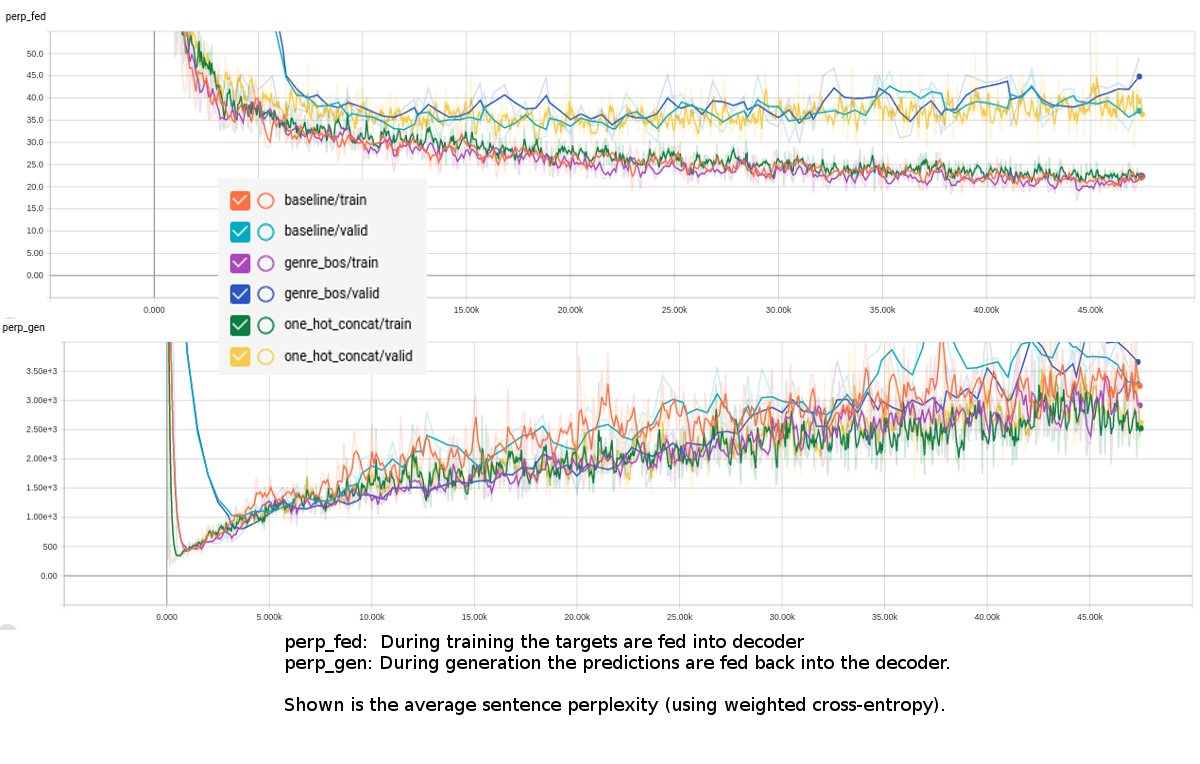
\includegraphics[width=0.95\textwidth, height=280px]{./img/perplexity.png}
%
\newline
%
 
As one can see in the graphs of the perplexities, our models did unfortunately not perform better than the baseline.
%
This result could be due to the fact that the model already had a hard time learning the language without the genre information. Adding the genre information would then not necessarily lead to an improvement.
%
Further, we do not see any performance difference between our extensions. We hoped that ensuring the influence of the genre in each step would perform better than the model where we replaced the $<$bos$>$ tag with a genre tag.
%
From this we conclude that either the genre does not have a significant impact on the form of the sentences, or that our implementation of the models was not able to fully use the genre information.
%
It would have been interesting to also test the model described in Section~\ref{mod:concat}, where an embedding of the gerne would be learned.
%
This would give the model a better representation of the genre tags, since the model will learn the embeddings in a context. These embeddings would only be affected by sentences of the correct genre, therefore containing information about the structure of a dialog in that genre.
%
\newline
%
Another observation is that the perplexities of the generated words are increasing with the iterations.
%
It makes sense that the perplexities of the generated words are worse than the perplexities of the mode where the targets are fed into the decoder. This is because the decoder, running in feedback mode, could "diverge" away from the correct targets, while the decoder in the other mode is held close to the targets. We do however not know why the perplexities are \emph{increasing}.
%
One possible explanation might be that the models are overfitting.